\titledquestion{Carpenter's Rule}

In this problem, you need to prove is $\mathsf{Carpenter}$ in $\complete{\NP}$.

$\mathsf{Carpenter}$: Given an array \(L=[l_1,l_2,\cdots,l_n]\) of non-negative integers, determine whether there exists a sequence $D=[d_1,d_2,\cdots,d_n]$ where $d_i\in\{\pm 1\}$ such that $\max_{j=0}^n\{\sum_{i=1}^{j}d_il_i\}-\min_{j=0}^n\{\sum_{i=1}^{j}d_il_i\}\leq k$.

Intuitively speaking, give a sequence of rigid rods of various integral lengths connected end-to-end by hinges, can it be folded so that its overall length is at most $k$? Correspondingly, $l_i$ indicates the length of $i$-th rigid rod and $d_i$ indicates the direction of $i$-th rigid rod (fold left or right). The $\max$ and $\min$ indicate the leftmost and rightmost positions.

\begin{figure}[H]
    \centering
    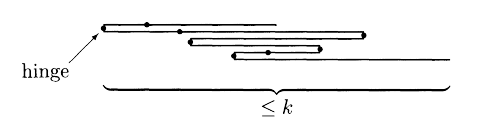
\includegraphics[width=0.5\linewidth]{hinge.png}
    \caption{Example of Hinge}
\end{figure}

The $yes$-instances of $\mathsf{Carpenter}$ is:
\begin{equation*}
\mathsf{Carpenter}= \left\{\langle{l_1, \ldots, l_{n},k\rangle}~\middle|~~~
\begin{aligned}
    & n\in \mathbb{Z}^+, l_1, \ldots, l_{n},k\in \mathbb{N},\exists D=[d_1,d_2,\cdots,d_n], d_i\in\{\pm 1\} \\ 
    & \text{i.e. }  D\in \{1,-1\}^{n} \text{ s.t. } \max_{j=0}^n\{\sum_{i=1}^{j}d_il_i\}-\min_{j=0}^n\{\sum_{i=1}^{j}d_il_i\}\leq k.
\end{aligned}
\right\}
\end{equation*}

\noindent We choose $\mathsf{Equivalent \text{-} Partition}$ to reduce from. Here is the $yes$-instance of it:
\begin{equation*}
\mathsf{Equivalent \text{-} Partition}= \left\{\langle{b_1, \ldots, b_{m}\rangle}~\middle|~~~\begin{aligned}
    &n\in \mathbb{Z}^+, b_1, \ldots, b_{m}\in \mathbb{N} \text{ and there exists a} \\ &\text{partition of the $b_i$'s to two parts whose sums}\\ &\text{are equivalent, i.e. }\exists{\:T\subseteq [m]}: \sum_{i\in T} b_i =  \sum_{j\in [m] \setminus T} b_j
\end{aligned}\right\}
\end{equation*}
Recall the definition of $\mathsf{Equivalent \text{-} Partition}$:

$\mathsf{Equivalent \text{-} Partition}$: Given an array \(B=[b_1,b_2,...,b_n]\) of non-negative integers, determine whether there exists a subset $T \subseteq [n]$ such that $\sum_{i\in T} b_i = \sum_{j \in [n] \setminus T} b_j $ (i.e. determine whether there is a way to partition $B$ into two disjoint subsets such that the sum of the elements in each subset is equivalent). 
\newpage
\begin{parts}
    \part[2] Prove that $\mathsf{Carpenter}$ is in $\NP$. (Show your certificate and certifier.)
    \begin{solution}\\
    Our certificate and certifier for $\mathsf{Carpenter}$ goes as follows:
    \begin{itemize}
        \item Certificate: 
        \item Certifier: 
    \end{itemize}
    \end{solution}

\part 
Consider how to construct your polynomial-time many-one reduction $f$ that maps instances of $\mathsf{Equivalent \text{-} Partition}$ to instances of $\mathsf{Carpenter}$. Unfortunately, the following reductions are not correct. Show that they are wrong by counterexamples.
\begin{subparts}
    \subpart[1] HaraoClesc gives out a reduction as follows: \\
    Let $n=m$ and $L=[l_1,l_2,\dots,l_n]$ be the sorted version in ascending order of $B=[b_1,\dots,b_m]$ i.e. $l_1$ is the minimum one in $B$, $a_n$ is the maximum of in $B$ and $l_i$ is the $i$-th minimum one in $B$ and $k = \frac12 \sum_{i=1}^{n}b_i$. Then $\aseq{l_1,\ldots,l_n,k}$ is a $yes$-instance of $\mathsf{Carpenter}$ if and only if $\aseq{b_1, b_2, \ldots, b_m}$ is a $yes$-instance of $\mathsf{Equivalent \text{-} Partition}$. 
    \begin{solution}\\\\
        \\
        \\
        \\
    \end{solution}
    \subpart[1] GeniusIdaiyo gives out another reduction as follows:
    Let $n=m+2$, then
        $$\aseq{l_1, \ldots, l_{n},k} = f(\aseq{b_1,\ldots,b_m}) \overset{\Delta}{=} \aseq{\max\{B\},b_1,\ldots,b_m,\max\{B\},\max\{B\}}$$ He deduces that $\aseq{l_1,\ldots,l_n,k}$ is a $yes$-instance of $\mathsf{Carpenter}$ if and only if $\aseq{b_1, b_2, \ldots, b_m}$ is a $yes$-instance of $\mathsf{Equivalent \text{-} Partition}$.
    \begin{solution}\\\\
\\
\\
\\
    \end{solution}
\end{subparts}
\newpage
\part From those wrong reductions above, FHKQ obtains a correct polynomial-time many-one reduction $f$ that maps instances of $\mathsf{Equivalent \text{-} Partition}$ to instances of $\mathsf{Carpenter}$. Show
\begin{subparts}
    \subpart[2] Your reduction in the format of (b).ii. (Show both $n$ and $L$.)\\
    \textbf{Hint:} Try to modify the above reductions into the correct one.
    \begin{solution}
\\
\\
\\
\\
\\
    \end{solution}
    \subpart[2]$x$ is a yes-instance of $\mathsf{Equivalent \text{-} Partition}\Rightarrow f(x)$ is a yes-instance of $\mathsf{Carpenter}$.
    \begin{solution}
\\
\\
\\
\\
\\
\\
\\
\\
\\
\\
\\
    \end{solution}
    \subpart[2]$f(x)$ is a yes-instance of $\mathsf{Carpenter}\Rightarrow x$ is a yes-instance of $\mathsf{Equivalent \text{-} Partition}$. 
    \begin{solution}
\\
\\
\\
\\
\\
\\
\\
\\
\\
\\
\\
    \end{solution}
\end{subparts}
\end{parts}



